%! Author = mariuszindel
%! Date = 25.01.21

\section{Leitungscodierung}

\subsection{Übersicht}
\subsubsection{Nur Nullstellen}
    \begin{tabular}{|l|l|l|l|l|}
        \hline
        \multirow{2}{*}{Leitungscode} & \multicolumn{2}{l|}{DC-Freiheit} & \multicolumn{2}{l|}{Taktinf} \\ \cline{2-5}
        & Ja             & Nein            & Ja               & Nein              \\ \hline
        Bipolarer NRZ            &                & X               &                  & X                 \\ \hline
        Unipolarer NRZ           & X               &                &                 &  X                 \\ \hline
        Unipolarer NRZ Mark      & *              &  *               &                 &  X                 \\ \hline
        Bipolarer Manchester     & X              &                 & X                &                   \\ \hline
        Unipolarer Manchester    &               &  X               & X                &                   \\ \hline
        Bipolarer AMI            & X              &                 &                 &  X                 \\ \hline
        Unipolarer RZ			 &	X			  & 			   & 				&	X				\\ \hline
    \end{tabular}
*Nicht entscheidbar kommt auf vorheriges Zeichen an

\subsubsection{Nur Einsstellen}
    \begin{tabular}{|l|l|l|l|l|}
        \hline
        \multirow{2}{*}{Leitungscode} & \multicolumn{2}{l|}{DC-Freiheit} & \multicolumn{2}{l|}{Taktinf} \\ \cline{2-5}
        & Ja             & Nein            & Ja               & Nein              \\ \hline
        Bipolarer NRZ            &                & X               &                  & X                 \\ \hline
        Unipolarer NRZ           &                & X               &                  & X                 \\ \hline
        Unipolarer NRZ Mark      & X              &                 & X                &                   \\ \hline
        Bipolarer Manchester     & X              &                 & X                &                   \\ \hline
        Unipolarer Manchester    & X              &                 & X                &                   \\ \hline
        Bipolarer AMI            & X              &                 & X                &                   \\ \hline
        Unipolarer RZ			 &				  & X		       & X				&					\\ \hline
    \end{tabular}

\subsubsection{Unipolarer Non-Return-to-Zero Code (NRZ)}
\begin{center}
    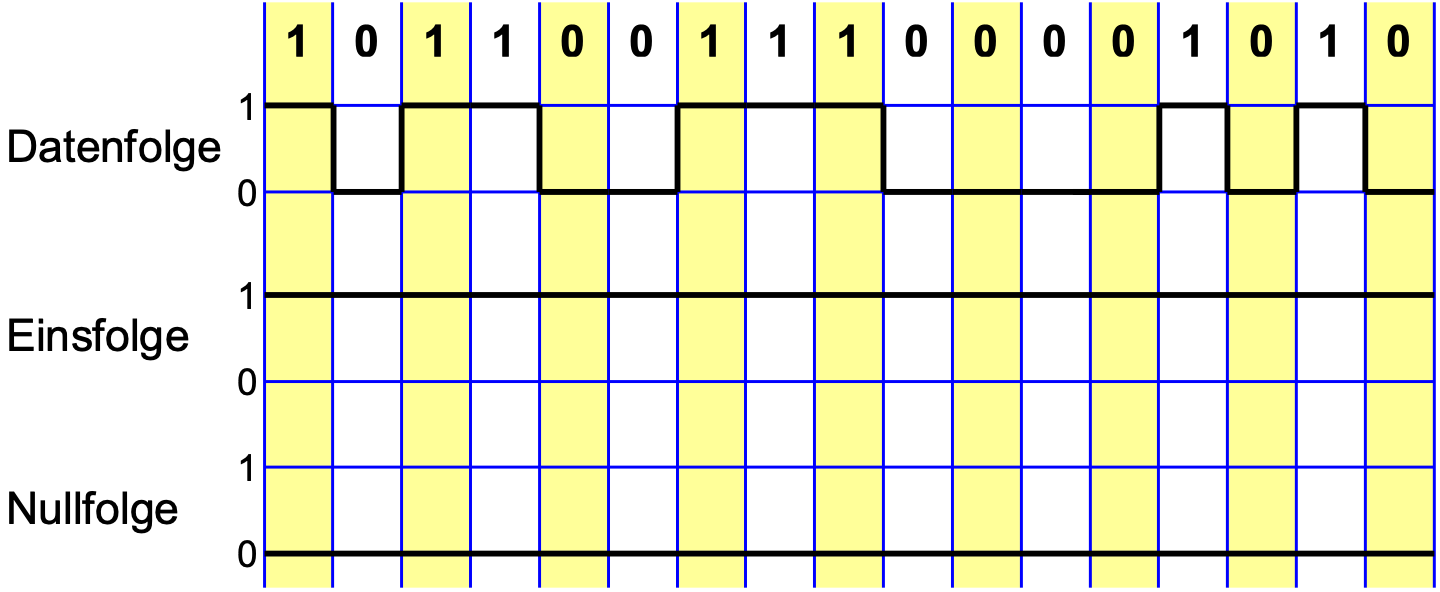
\includegraphics[width=\linewidth]{graphic/signale_analyisieren/Unipolarer Non-Return-to-Zero Code (NRZ).png}
\end{center}
\vspace{-8pt}
\begin{itemize}
    \item Gleichspannungsanteil, auch bei Random-Daten
    \item Verlust des Taktes bei langen Eins- und Nullfolgen
    \item Datenfolge enthält nicht direkt Frequenzanteile bei der Taktfrequenz
\end{itemize}


\subsubsection{Bipolarer Non-Return-to-Zero Code (NRZ)}
\begin{center}
    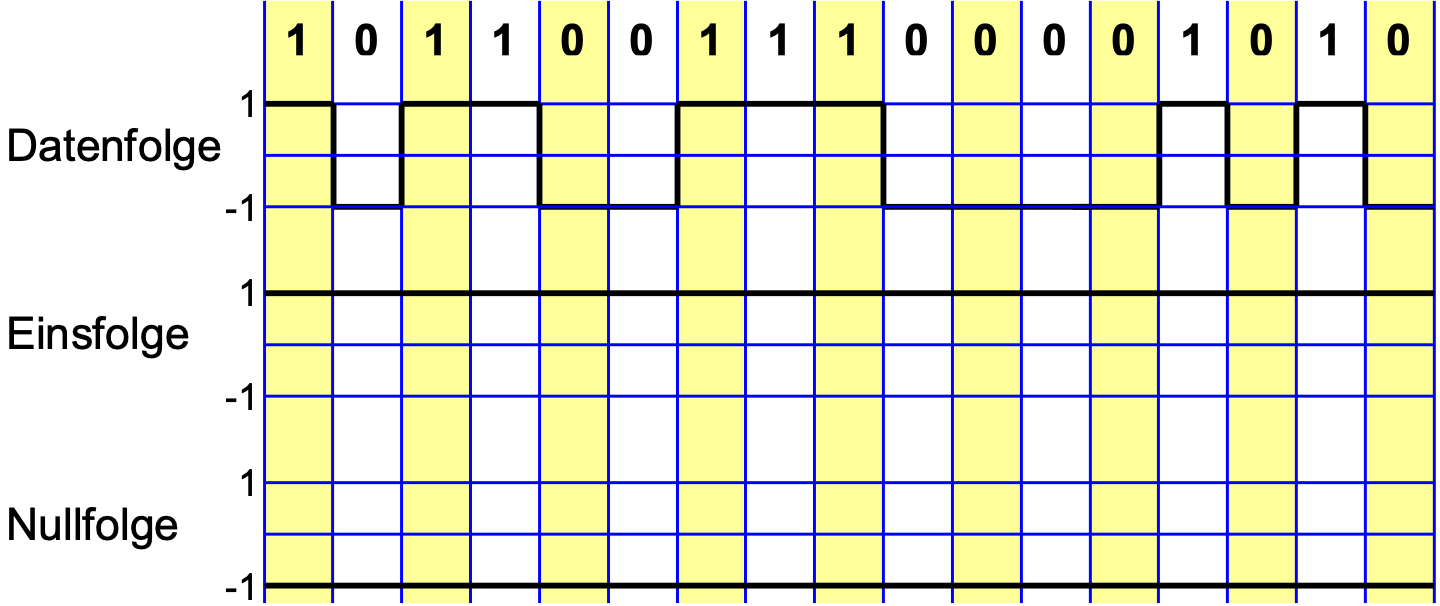
\includegraphics[width=\linewidth]{graphic/signale_analyisieren/Bipolarer Non-Return-to-Zero Code (NRZ).png}
\end{center}
\vspace{-8pt}
\begin{itemize}
    \item Kein Gleichspannungsanteil bei Random-Daten
    \item Gleichspannungsanteil bei langen Eins- und Nullfolgen
    \item Verlust des Taktes bei langen Eins- und Nullfolgen
\end{itemize}


\subsubsection{NRZ Mark Code  (Differentielle Codierung)}
\begin{center}
    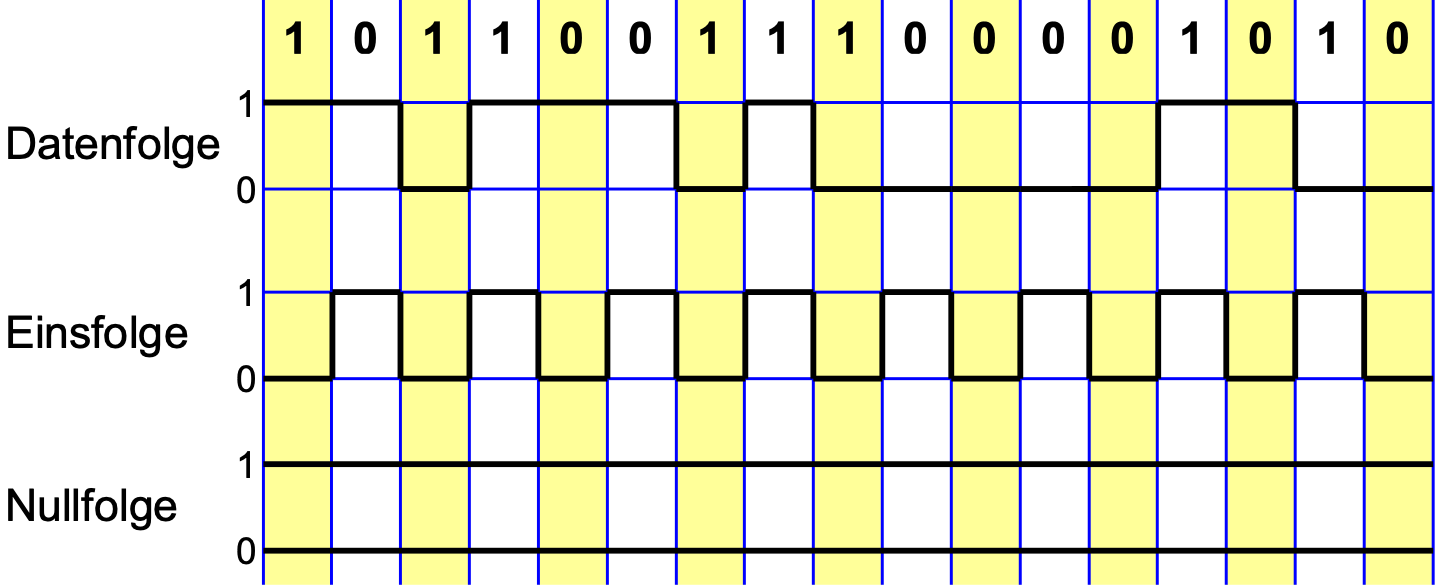
\includegraphics[width=\linewidth]{graphic/signale_analyisieren/NRZ Mark Code Differentielle Codierung.png}
\end{center}
\vspace{-8pt}
\begin{itemize}
    \item Robust gegen Vertauschen der Polarität (a/b Klemmen, absolute Phasenlage)
    \item Verlust des Taktes bei langen Nullfolgen
\end{itemize}


\subsubsection{Return-to-Zero Code (RZ)}
\begin{center}
    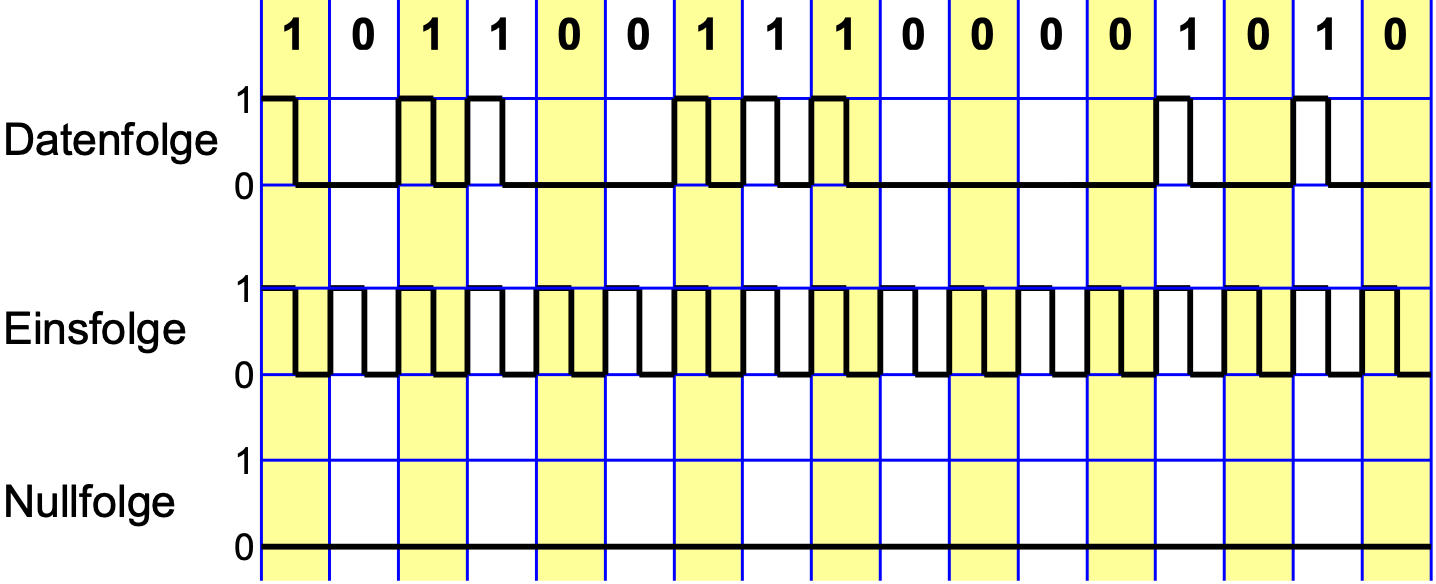
\includegraphics[width=\linewidth]{graphic/signale_analyisieren/Return-to-Zero Code (RZ).png}
\end{center}
\vspace{-8pt}
\begin{itemize}
    \item Datensignal enthält direkt Frequenzanteile bei der Taktfrequenz
    \item Durch Halbierung der Bitdauer Verdoppelung des Bandbreitenbedarfs
    \item Verlust des Taktes bei langen Nullfolgen
\end{itemize}


\subsubsection{Bi-Phase oder Manchester Code (Ethernet)}
\begin{center}
    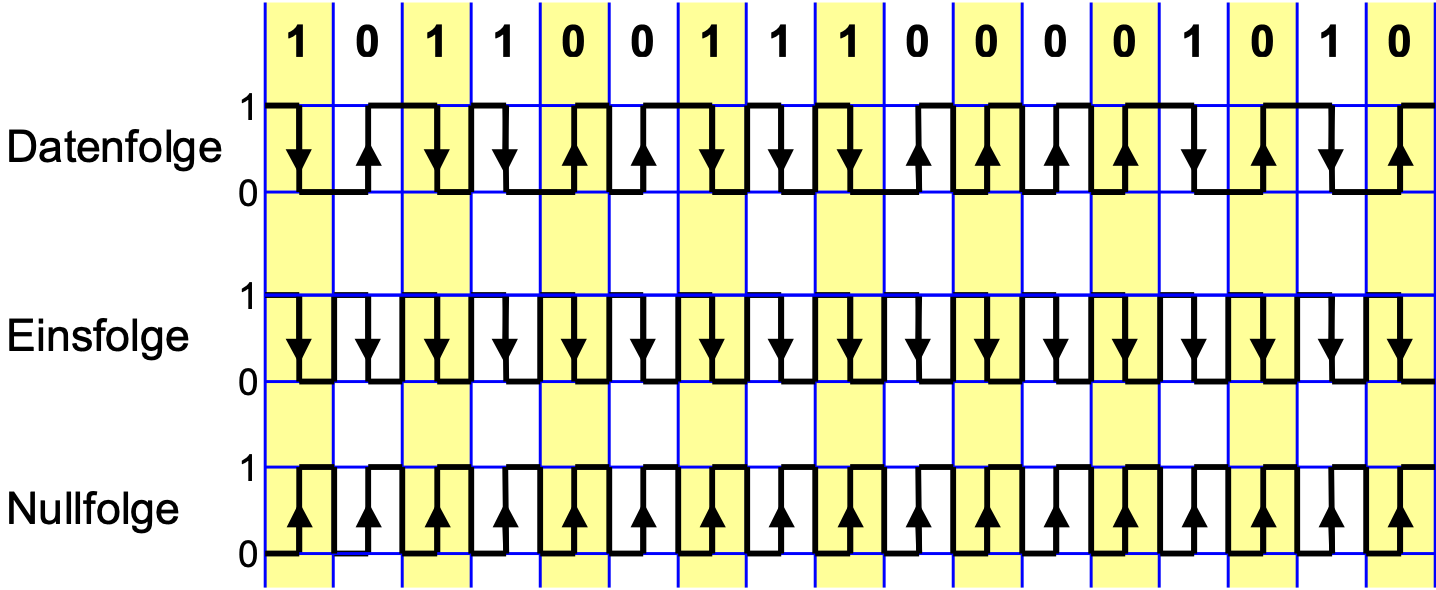
\includegraphics[width=\linewidth]{graphic/signale_analyisieren/Bi-Phase oder Manchester Code.png}
\end{center}
\vspace{-8pt}
\begin{itemize}
    \item Takt ist in jedem Datenbit vorhanden
    \item Bei bipolarem Code ist jedes Datenbit gleichspannungsfrei
    \item Durch Halbierung der Bitdauer Verdoppelung des Bandbreitenbedarfs
\end{itemize}

\subsubsection{Alternate Mark Inversion Code (AMI)}
\begin{center}
    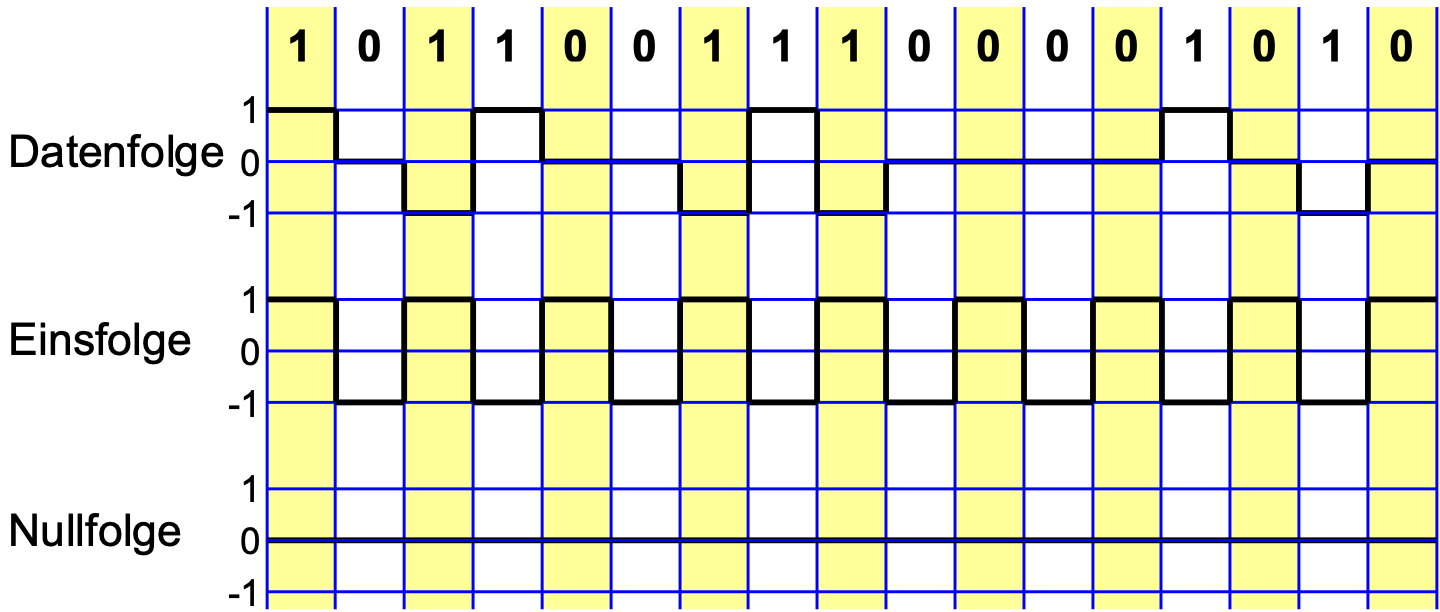
\includegraphics[width=\linewidth]{graphic/signale_analyisieren/Alternate Mark Inversion Code (AMI).png}
\end{center}
\vspace{-8pt}
\begin{itemize}
    \item Ternärer Code mit drei Spannungspegel
    \item Dank Alternierung Gleichspannungsfreiheit
    \item Verlust des Taktes bei langen Nullfolgen
\end{itemize}


\subsubsection{Scrambling}
\begin{center}
    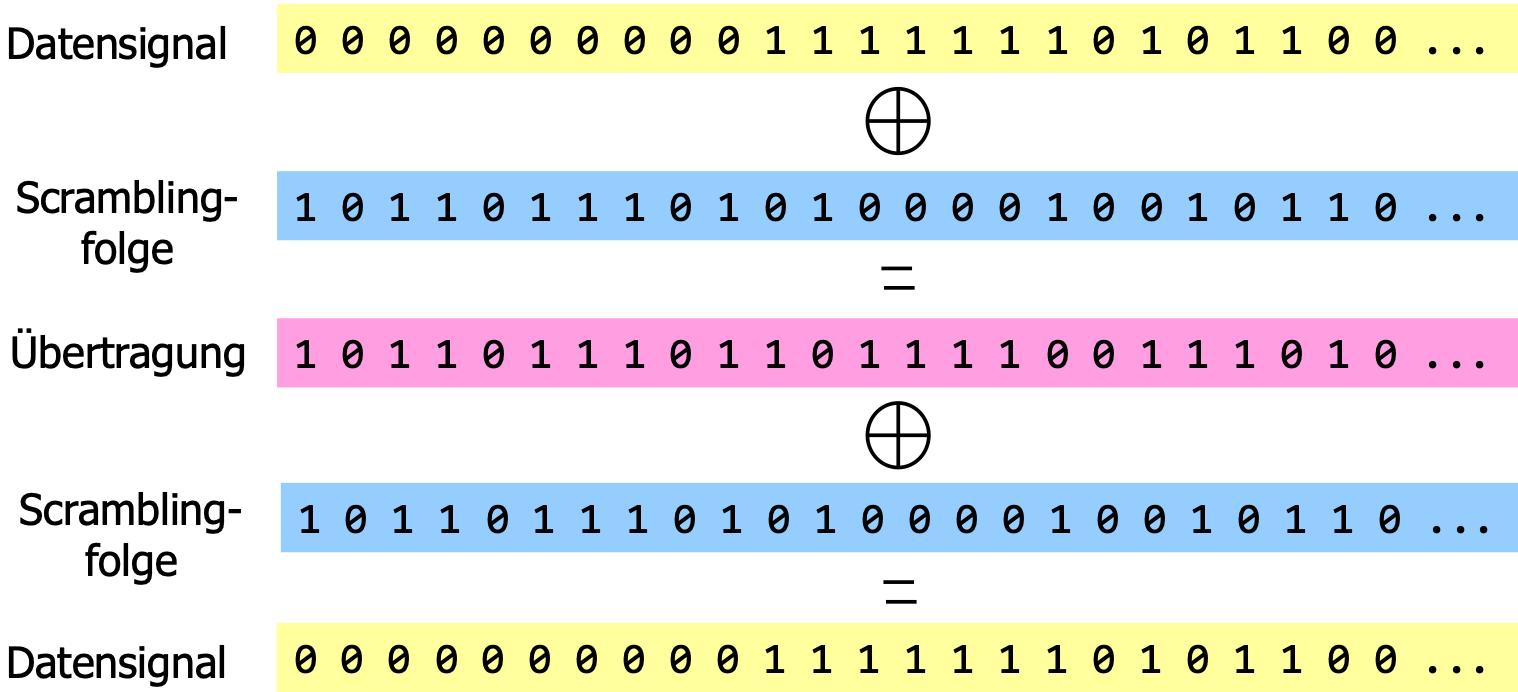
\includegraphics[width=\linewidth]{graphic/signale_analyisieren/Scrambling.png}
\end{center}
\vspace{-8pt}
\begin{itemize}
    \item Pseudozufällige Scramblingfolge z.B. aus rückgekoppeltem Schieberegister
    \item Eliminierte lange Null- und Einsfolgen
    \item Scrambler-Synchronisation setzt meist Rahmenstruktur der Daten voraus
\end{itemize}



%\section{Zweiseitiges Spektrum}
%TODO